\section{Experiments and Analysis}
\label{sec:experiments}

To substantiate the claims of our method's effectiveness and superiority, we conduct a comprehensive suite of experiments. This section first outlines the implementation details and evaluation protocols. We then present extensive qualitative and quantitative comparisons against state-of-the-art methods to demonstrate our model's advanced capabilities. Finally, we perform detailed ablation studies to validate our architectural choices and analyze key parameters to showcase the model's controllability.

\subsection{Experimental Setup}
\label{subsec:setup}



\noindent\textbf{Training Dataset.}
Our model is trained on the Subject-Materials-Style-Set (SMSS), a style-balanced dataset we curated. To ensure high-quality training pairs, we applied a LAION-Aesthetics threshold of 6.25 and a Semantic Consistency Filter (CLIP score $> 0.3$). Because image-text prompts often contain detailed style descriptions that entangle style and content, we removed all style-related descriptions from the text in SMSS, retaining only content-related text. This decoupled training strategy encourages the model to extract style solely from the reference images. To mitigate the stylistic bias typical of large datasets like LAION, we curated SMSS to be diverse and employed Category-Aware Uniform Sampling—uniformly sampling style categories before individual images—to ensure equal gradient updates even for rare styles (see Figure~\ref{fig:dataset_distribution}).

\begin{figure}[htbp]
\centering
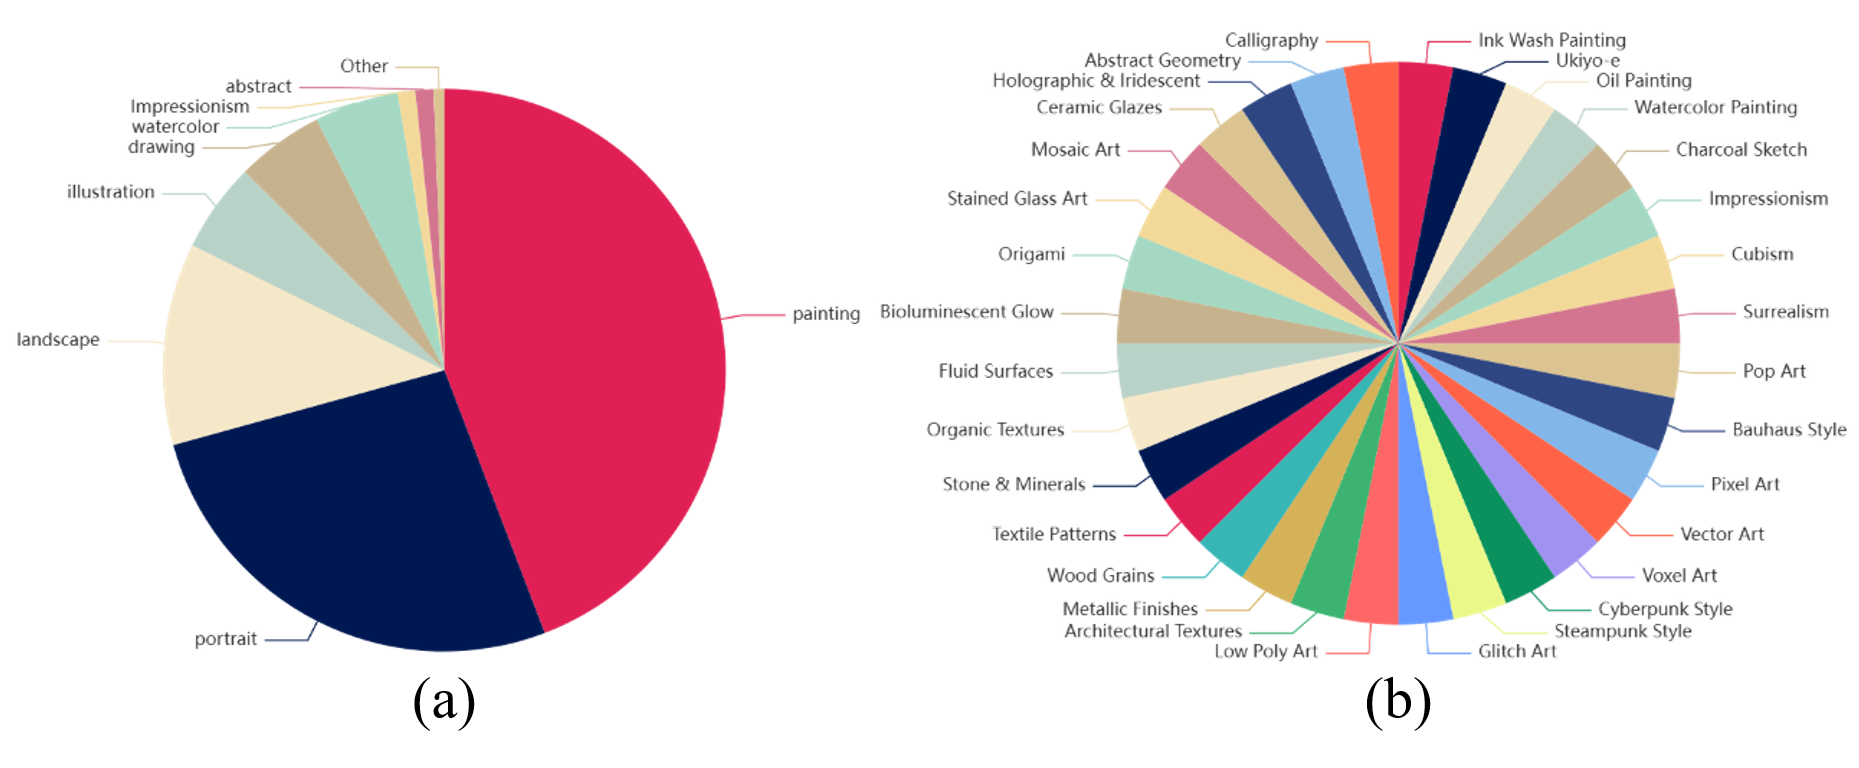
\includegraphics[width=1.0\columnwidth]{images/data.png}
\caption{Category distribution comparison. (a): LAION's skewed distribution. (b): Our SMSS dataset's uniform distribution across diverse styles, ensuring balanced training.}
\label{fig:dataset_distribution}
\end{figure}

\noindent\textbf{Test Datasets.}
Our experimental evaluation is grounded in widely adopted benchmarks to ensure fair and reproducible comparisons. We utilize the MS-COCO dataset~\cite{lin2014microsoft} for its diverse and high-quality content images, providing a robust testbed for content preservation. For style references, we employ the WikiArt dataset, whose vast collection of artistic styles serves as a comprehensive benchmark for evaluating stylization performance.



\noindent\textbf{Evaluation Metrics.}
We employ a set of well-established metrics to perform a multi-faceted and objective assessment of our model's performance.
\begin{itemize}
    \item \textbf{ArtFID}~\cite{wright2022artfid}, a composite metric ($ArtFID = (1 + LPIPS) \times (1 + FID)$), is used to measure the overall balance between content preservation (LPIPS) and style fidelity (FID). Lower scores indicate superior overall quality.
    \item \textbf{FID (Fr\'echet Inception Distance)}~\cite{heusel2017gans} quantifies the distributional similarity between generated images and the target style. For style transfer, FID is computed between 1,000 generated images and 1,000 images from the corresponding style set in WikiArt.
    \item \textbf{LPIPS (Learned Perceptual Image Patch Similarity)}~\cite{zhang2018perceptual} assesses perceptual similarity to the original content image, providing a precise measure of content preservation.
    \item \textbf{CLIP and DINO Scores}: To evaluate semantic alignment for material transfer, we report image-image similarity scores using CLIP (ViT-L/14) and DINOv2 (ViT-g/14) backbones. The reported values are cosine similarities multiplied by 100 for readability. We use CLIP for SDXL compatibility and additionally incorporate the CSD (Cross-domain Structural Distance) metric to comprehensively evaluate stylization performance.
\end{itemize}


\subsection{Implementation Details}
Our framework is built upon the \textbf{SDXL 1.0 base} model. For style feature extraction, we utilize the \textbf{OpenCLIP ViT-L/14} image encoder. Both models are kept frozen during the training of our Resampler network. The trainable Resampler network is a lightweight transformer consisting of \textbf{4 layers}, with each layer containing a multi-head self-attention block with \textbf{8 attention heads} and a feed-forward network. 
For all experiments, we use the \textbf{DPM++ 2M Karras} sampler with \textbf{25 inference steps}. The Classifier-Free Guidance (CFG) scale is set to \textbf{7.5}. To ensure a fair and robust evaluation, we standardized the textual prompts used during inference to the generic phrase: ``realistic, 4k, high definition, no watermarks.'' The style strength parameter, $\lambda_s$, is empirically set within the range of \textbf{0.6 to 0.8}, which we found to provide a good balance between style fidelity and content preservation.

\begin{figure*}[htbp]
    \centering
    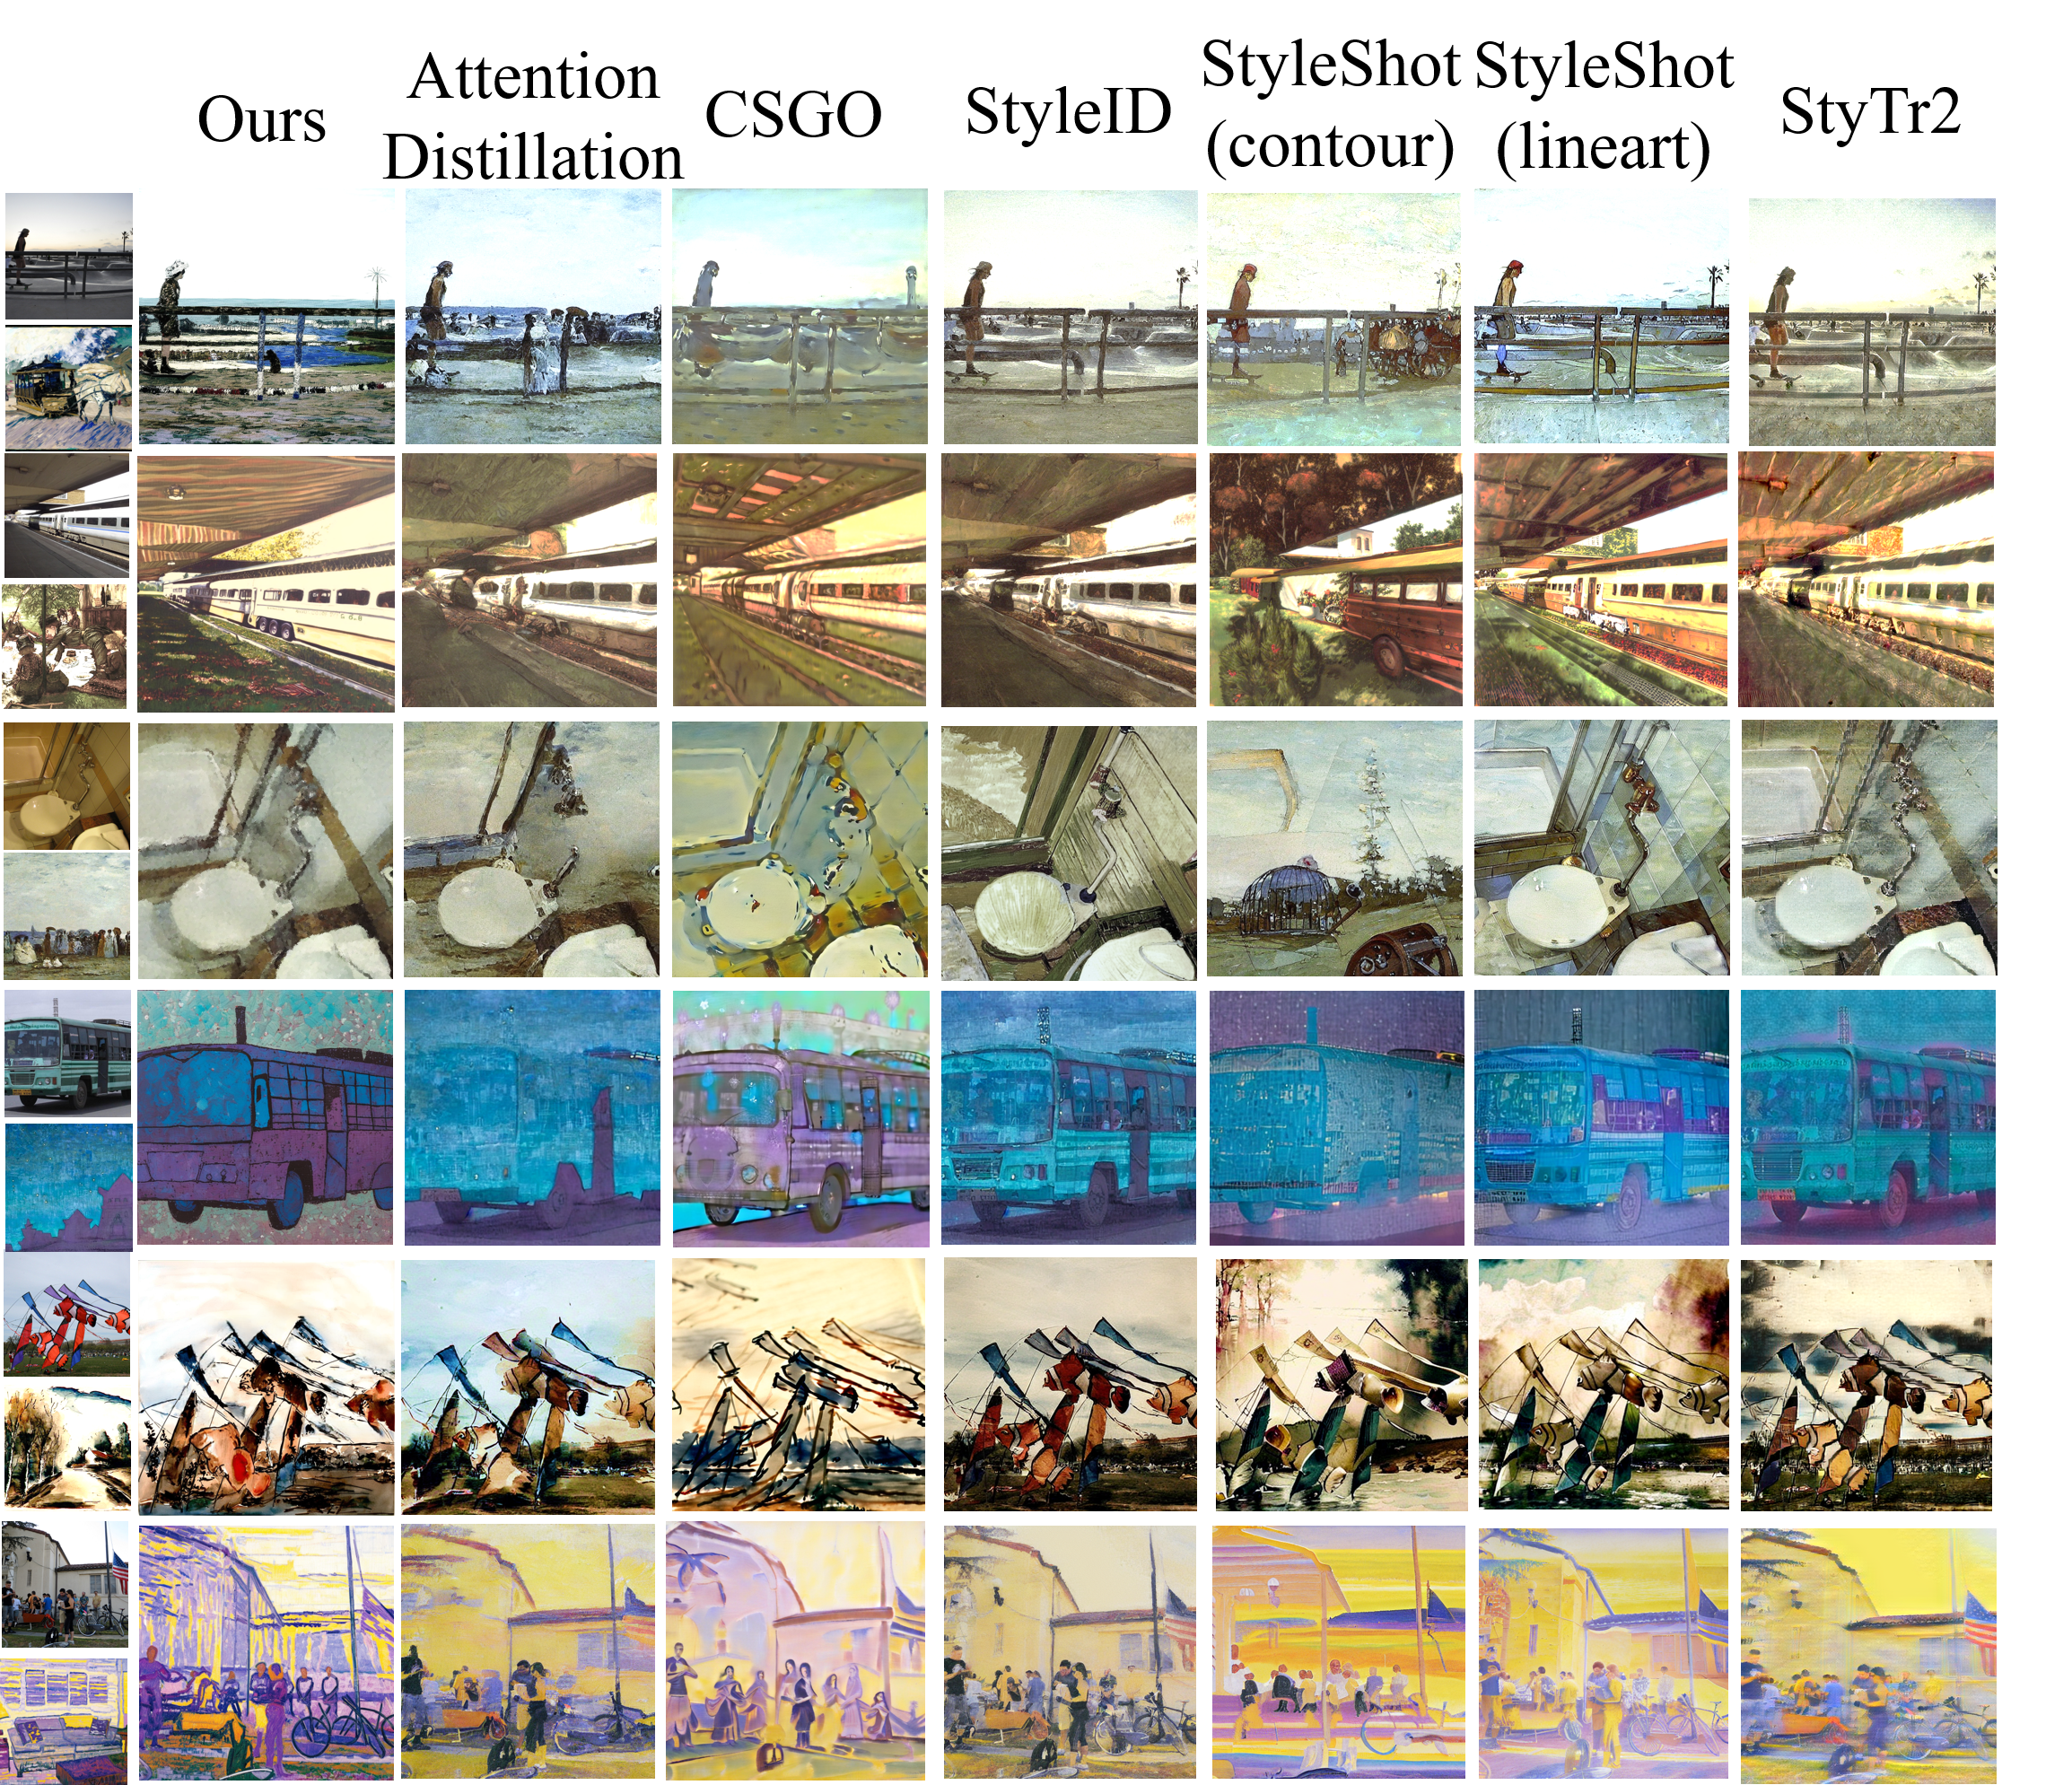
\includegraphics[width=1.0\textwidth]{images/style_transfer_comparison.png}
    \caption{Qualitative comparison for style transfer.}
    \label{fig:style_transfer_comparison}
\end{figure*}


\subsection{Qualitative Evaluation}
\label{subsec:qualitative}


We begin by visually demonstrating our method's proficiency in two challenging tasks: style and material transfer. The qualitative results presented here serve to provide intuitive evidence of our model's superiority in generating coherent, detailed, and aesthetically pleasing results.

\noindent\textbf{Style Transfer.}
As illustrated in Figure~\ref{fig:style_transfer_comparison}, we compare our method against a representative baseline. The visual evidence clearly shows that our approach not only captures the global ambiance of the style reference but also adeptly reproduces its fine-grained textural details and brushwork. While color matching in isolated cases might appear subtle, our priority is maintaining semantic consistency and structural integrity across diverse prompts. In contrast, the baseline struggles with artifacts and fails to achieve a comparable level of stylistic integration, highlighting the advanced capabilities of our model.

\begin{figure}[htbp]
    \centering
    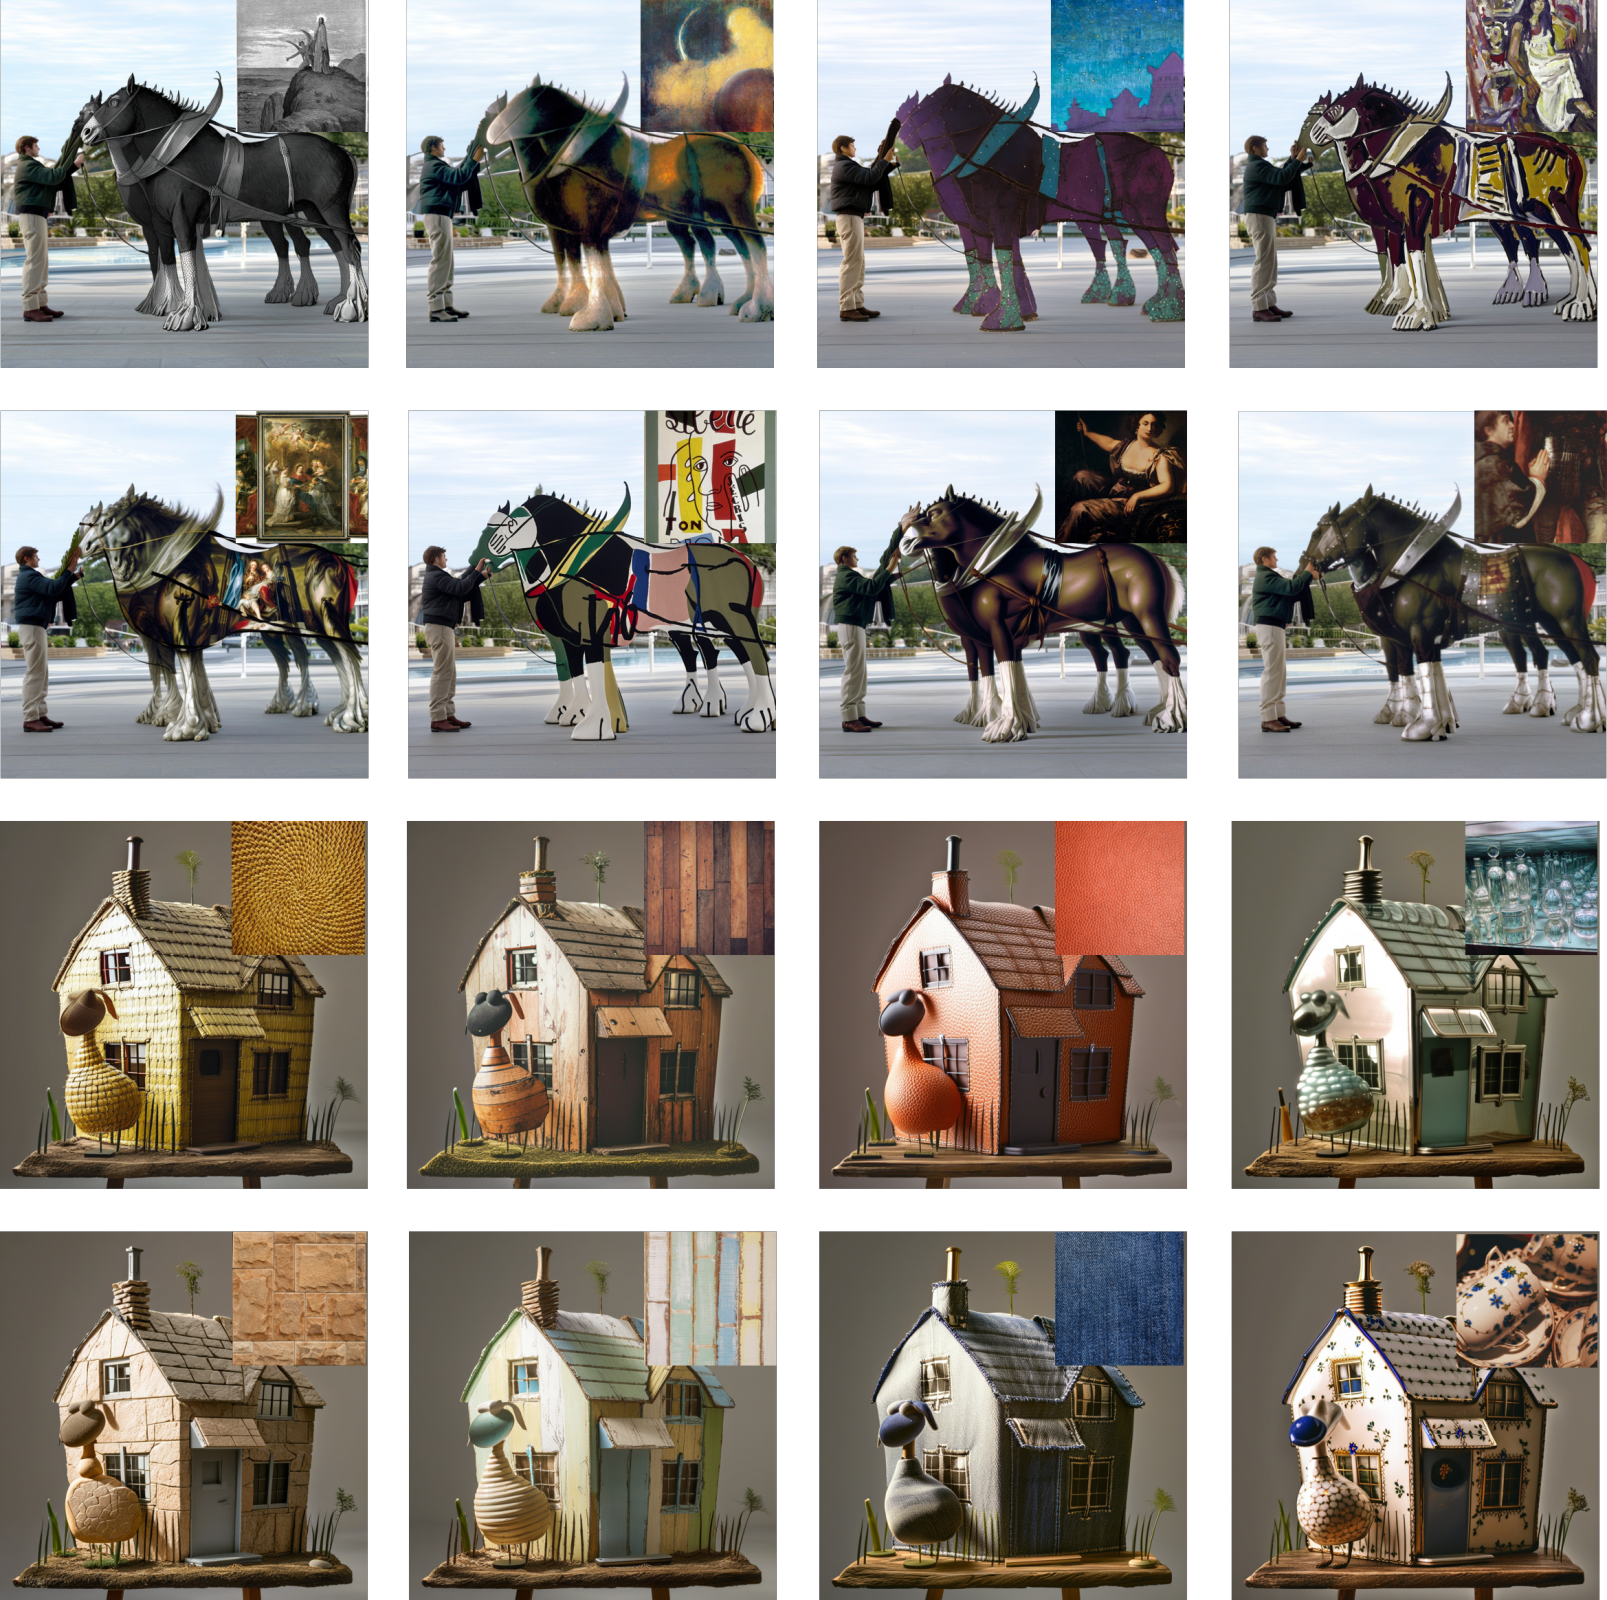
\includegraphics[width=1.0\columnwidth]{images/local.png}
    \caption{Demonstration of local style transfer on a masked region. Please zoom in for details.}
    \label{fig:local_transfer}
\end{figure}

\noindent\textbf{Local Style Transfer.}
Importantly, our framework is not limited to global stylization. As shown in Figure~\ref{fig:local_transfer}, it offers precise spatial control, enabling style application to specific masked regions. This capability for local manipulation is a significant advantage over many existing methods, allowing users to stylize only the targeted objects (e.g., the dress of the girl) while preserving the original appearance of the background. By restricting the style injection to the specified mask, our model seamlessly blends the stylized content with the unedited surroundings, demonstrating highly controllable and fine-grained editing capabilities.



\begin{figure}[htbp]
    \centering
    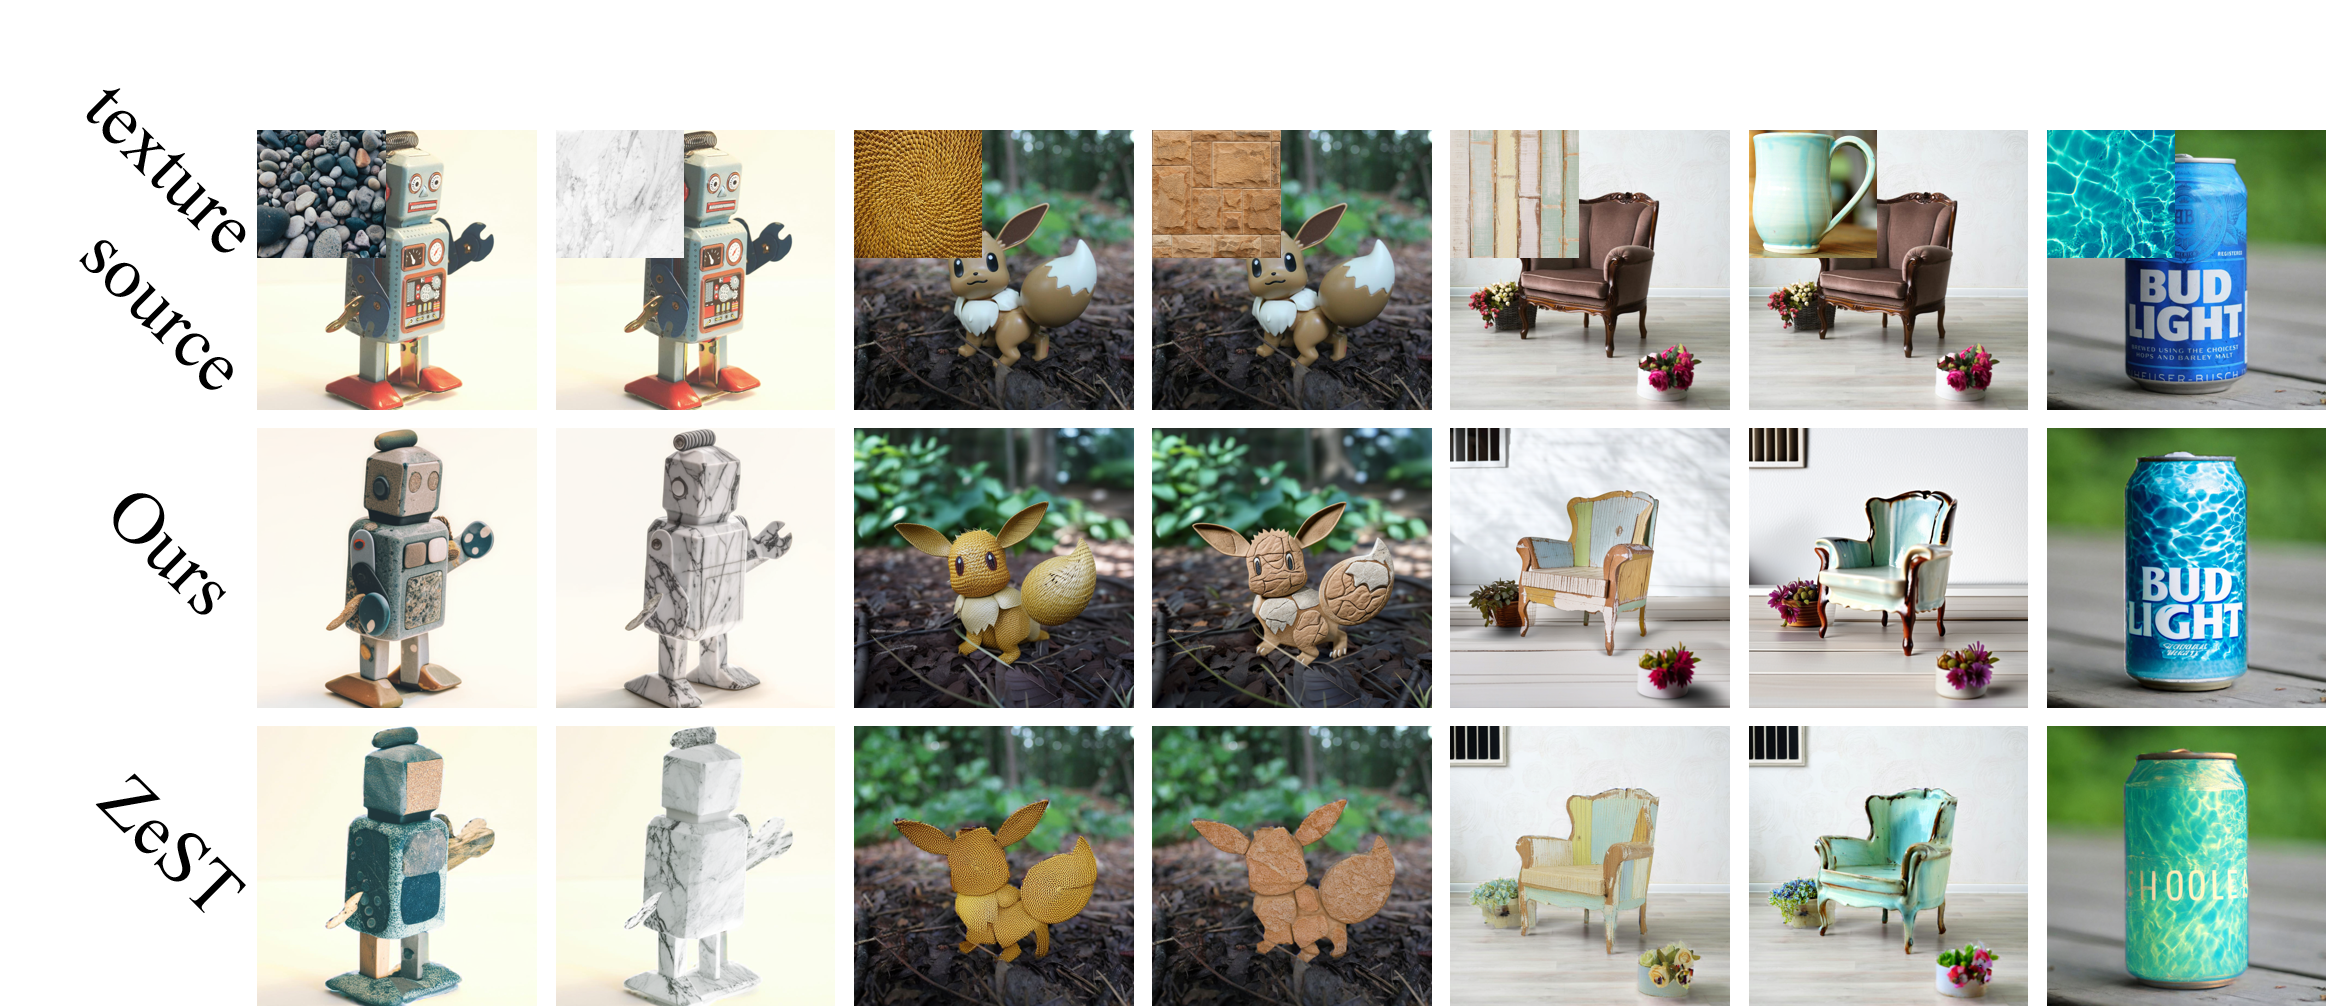
\includegraphics[width=1.0\columnwidth]{images/material_transfer_comparison.png}
    \caption{Qualitative comparison for material transfer against the ZeST baseline. Please zoom in for details.}
    \label{fig:material_transfer_comparison}
\end{figure}

\noindent\textbf{Material Transfer.}
To further probe the capabilities of our framework, we evaluate its performance on the demanding task of material transfer. Figure~\ref{fig:materials_transfer_display} provides a gallery of results, showcasing our model's versatility across a diverse set of materials and objects. The subsequent comparison in Figure~\ref{fig:material_transfer_comparison} against the representative method ZeST reveals the clear advantages of our approach. Our model generates textures with a markedly higher degree of photorealism, correctly conforming to the object's underlying structure and responding accurately to its lighting environment. This underscores our model's sophisticated understanding of the interplay between material, shape, and light.


\begin{figure}[htbp]
    \centering
    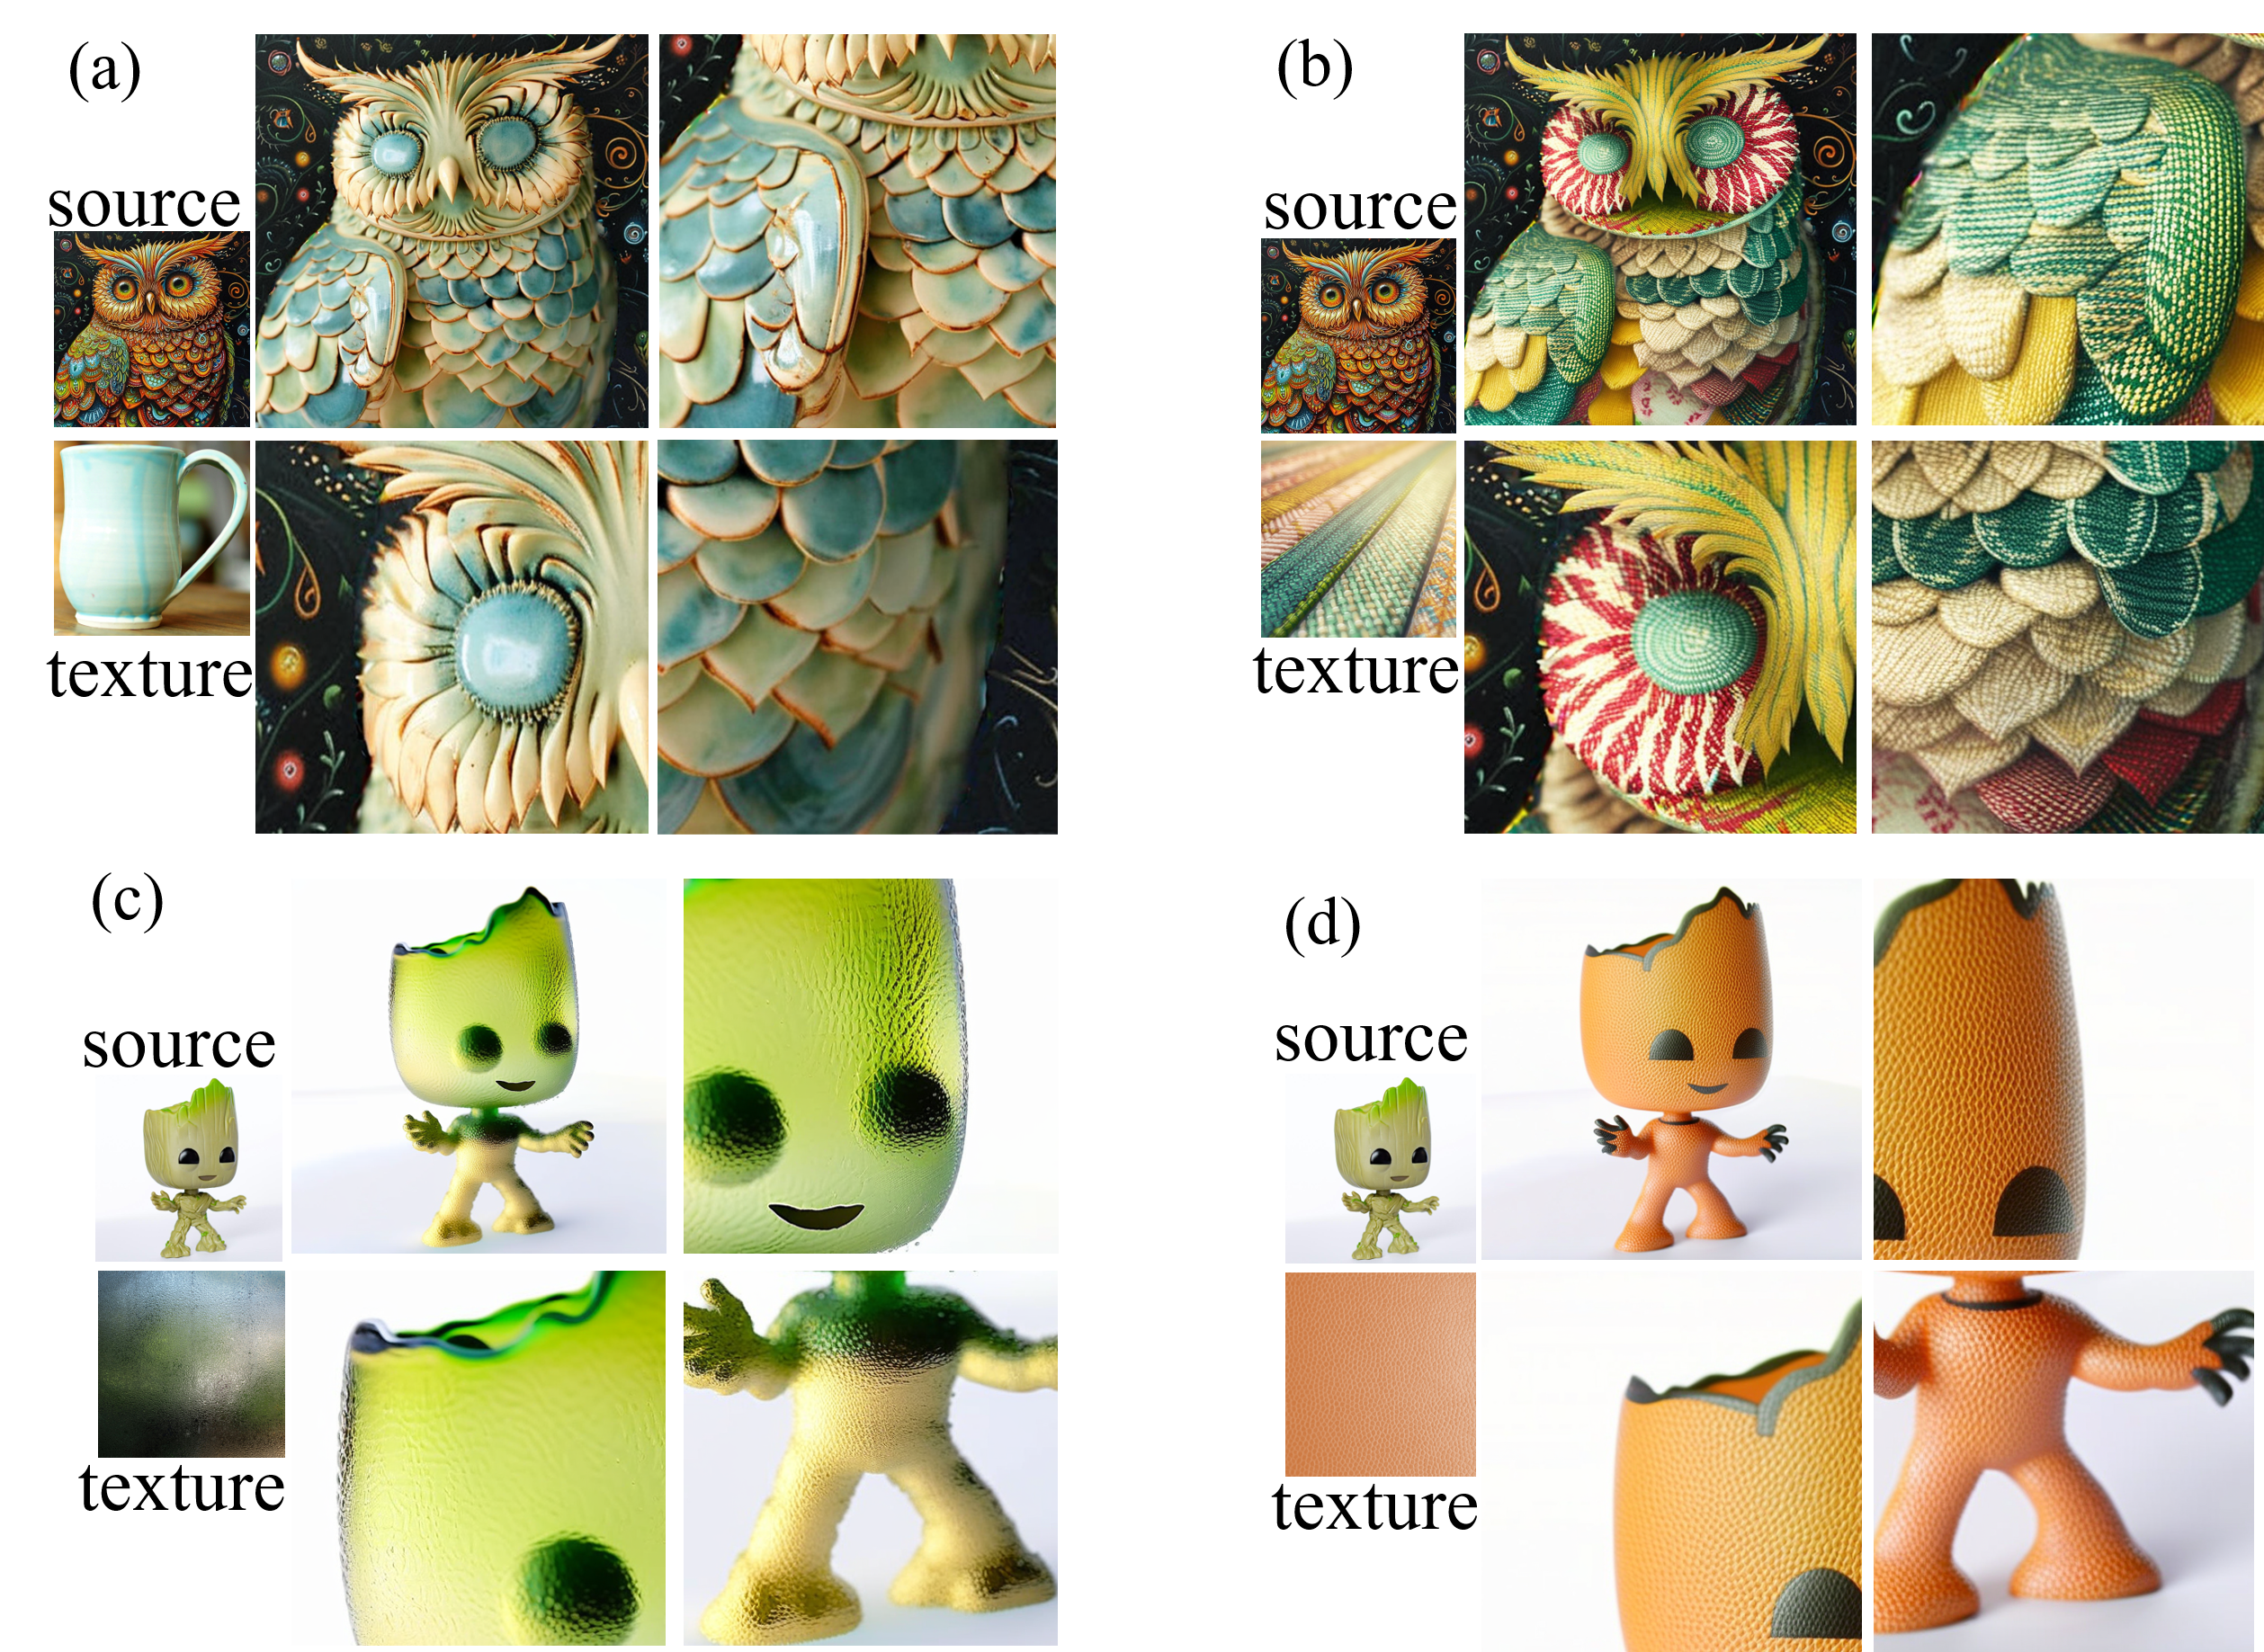
\includegraphics[width=1.0\columnwidth]{images/materials_transfer_display.png}
    \caption{Gallery of material transfer results. }
    \label{fig:materials_transfer_display}
\end{figure}


\begin{figure}[t!]
\centering
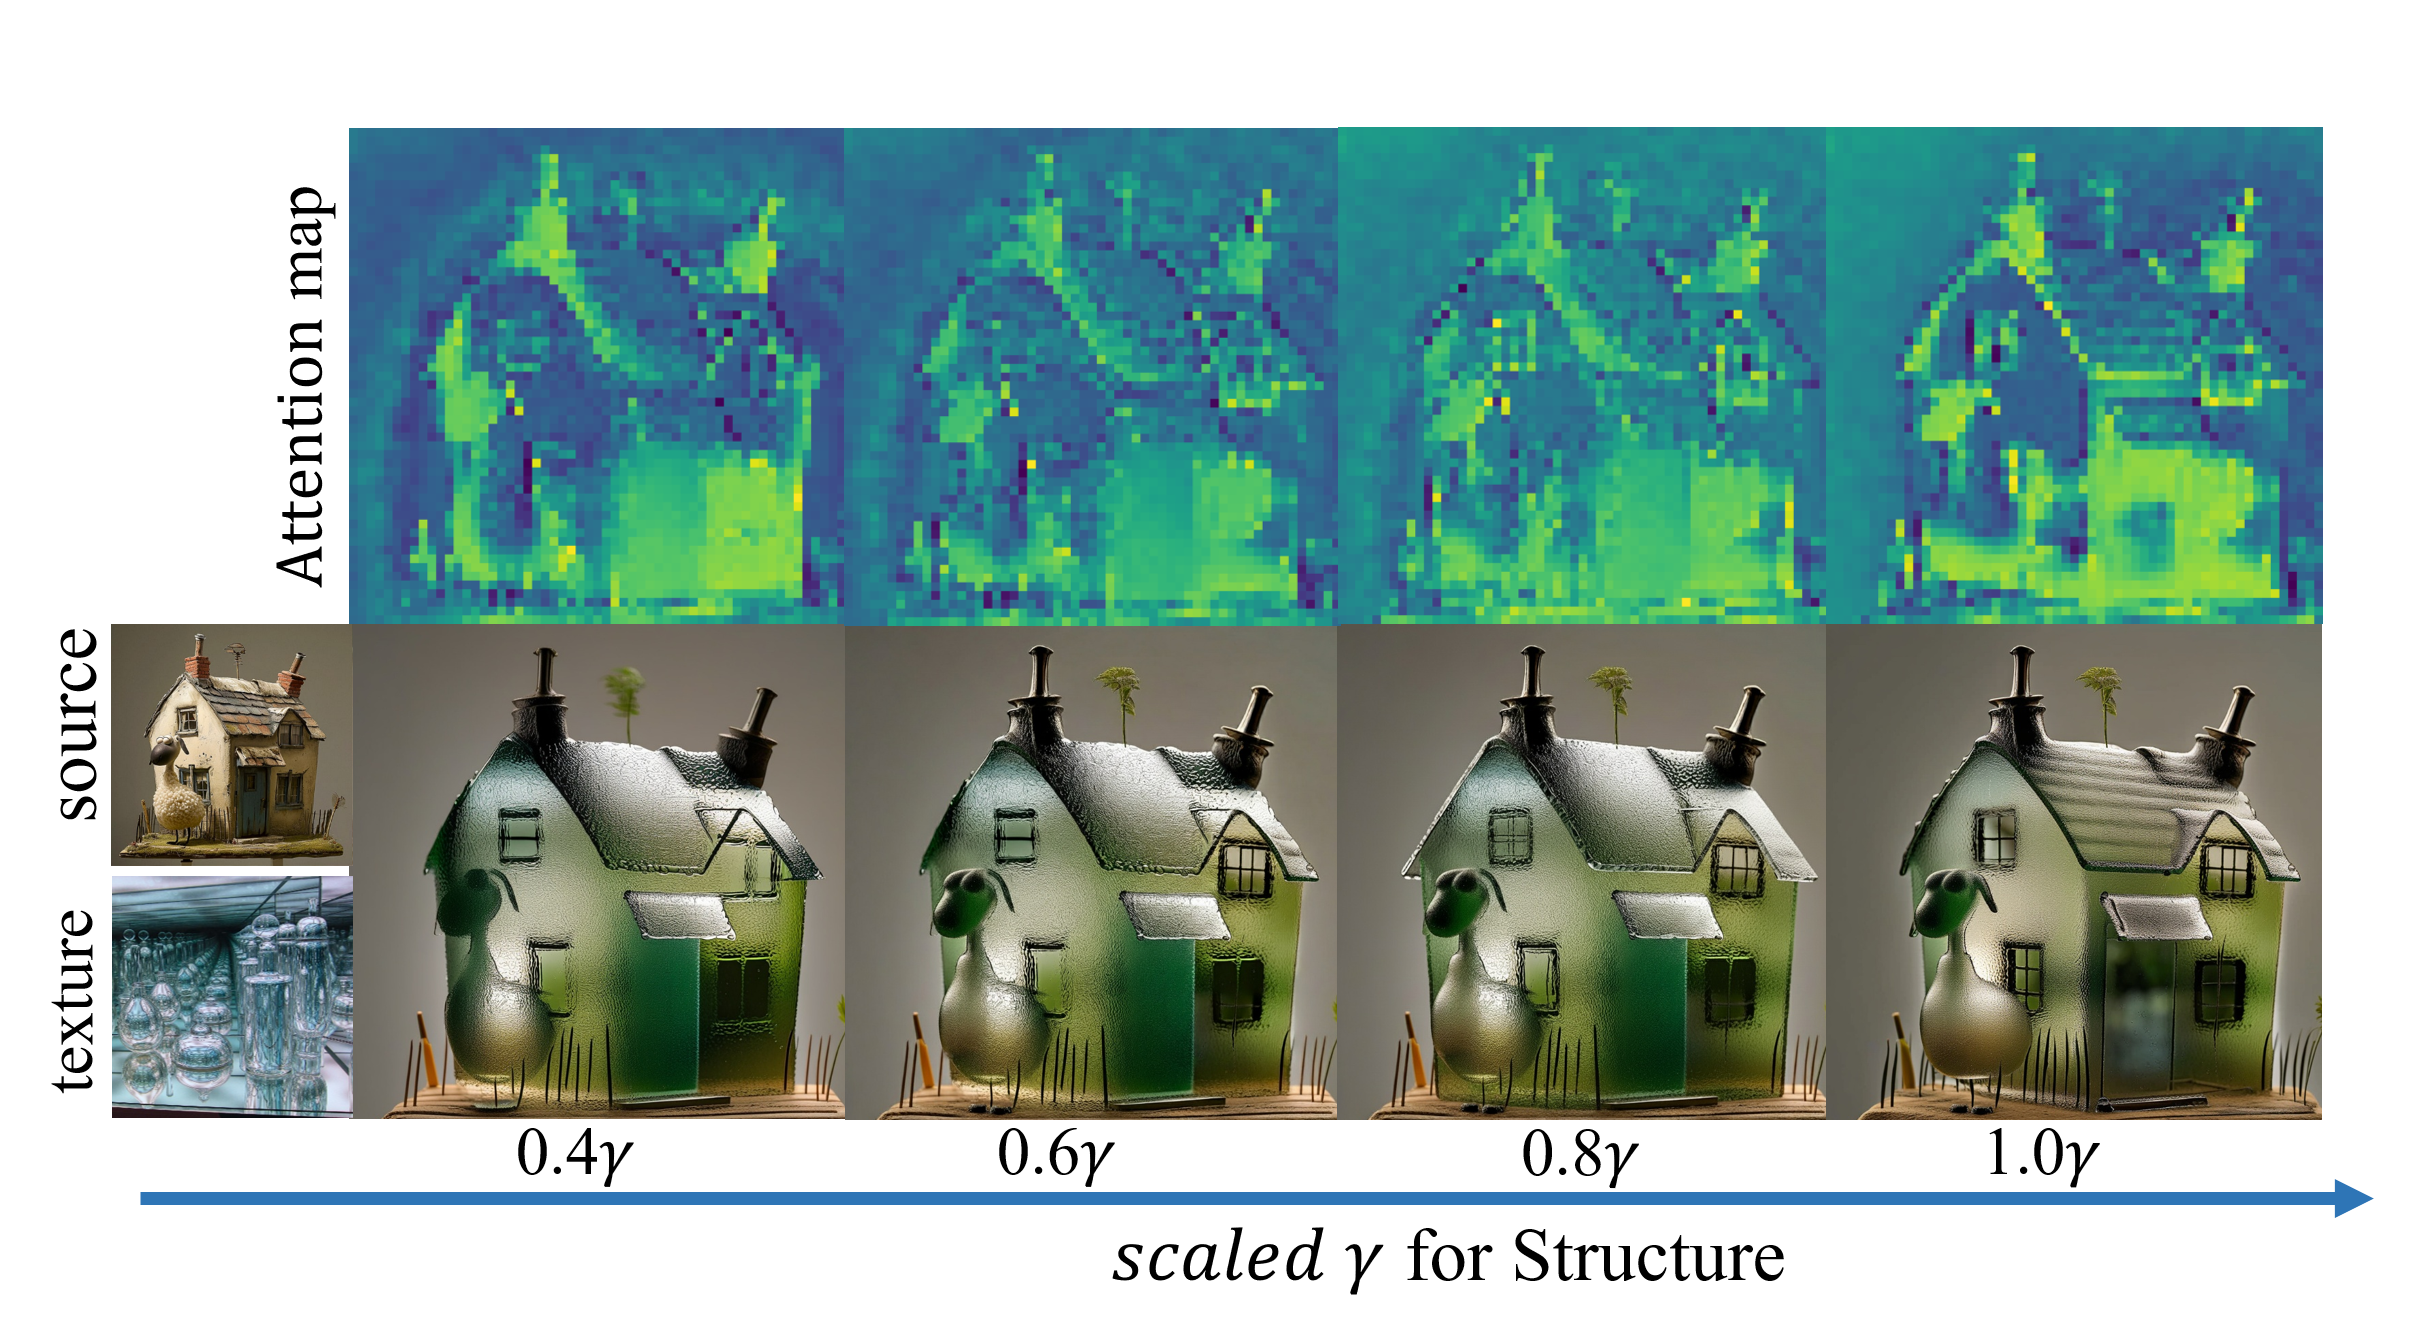
\includegraphics[width=1.0\columnwidth]{images/structure.png}
\caption{Material transfer results guided by varying strengths of structural control.}
\label{fig:structure}
\end{figure}

\subsection{Quantitative Analysis}
\label{subsec:quantitative}

To complement the qualitative evidence with objective, empirical data, we conduct a thorough quantitative analysis. We benchmark our method against several leading approaches and support our findings with a user study, providing a holistic evaluation of its performance.

\noindent\textbf{User Study.}
We conducted a user study with \textbf{187 participants} covering both style and material transfer tasks. Each participant rated method outputs on a \textbf{5-point Likert scale} across stylization quality and content preservation, yielding over \textbf{5,000 individual ratings}. Statistical significance was confirmed via the Wilcoxon signed-rank test ($p < 0.05$) against all baselines. Our method received the highest mean scores across all criteria.

\noindent\textbf{Style Transfer Evaluation.}
The quantitative results for style transfer are summarized in Table~\ref{tab:style_transfer_metrics}. Our method achieves the lowest LPIPS and LPIPS$_{gray}$ scores, signifying its SOTA capability for content preservation. While maintaining highly competitive FID and ArtFID scores, this strong content fidelity is crucial for practical applications. These empirical results are corroborated by the user study results, also included in the table, where our method received the highest rating for stylization quality, indicating a strong preference from human evaluators. Furthermore, to evaluate our model's capability in subject-driven style transfer, we conducted an automatic evaluation on the DreamBench++ benchmark, achieving excellent performance (see Appendix for details).

\begin{table*}[htbp]
\centering
\small
\begin{tabular}{lccccccc}
\toprule
Metric & CSGO & StyleShot(contour) & StyleShot(lineart)& StyTr2 & StyleID  & Attn. Distill. & \textbf{Ours} \\
\midrule
ArtFID ($\downarrow$) & 36.930 & 36.426 & 35.488 & 30.708 & 28.778 & 28.977 & \textbf{25.029} \\
FID ($\downarrow$) & 21.207 & 19.580 & 20.639 & 18.889 & 18.122 & 17.504 & \textbf{16.877} \\
LPIPS ($\downarrow$) & 0.663 & 0.770 & 0.640 & 0.544 & 0.505 & 0.566 & \textbf{0.483} \\
$LPIPS_{gray}$ ($\downarrow$) & 0.539 & 0.683 & 0.529 & 0.449 & 0.439 & 0.470 & \textbf{0.433} \\
\midrule
User Preference ($\uparrow$) & 4.0 & 3.2 & 3.9 & 4.1 & 4.3 & 3.8 & \textbf{4.5} \\
\bottomrule
\end{tabular}

\caption{Quantitative comparison and user study for style transfer. For objective metrics, ($\downarrow$) indicates lower is better. For the user study, ($\uparrow$) indicates higher is better.}
\label{tab:style_transfer_metrics}
\end{table*}

\noindent\textbf{Material Transfer Evaluation.}
For the material transfer task, our method's superiority is even more pronounced. As shown in Table~\ref{tab:material_transfer_metrics}, our approach significantly outperforms the ZeST baseline across all objective metrics. The substantial gains in CLIP and DINO scores point to a much stronger alignment of high-level semantic features. This conclusion is further reinforced by the user study results, where our method earned substantially higher scores for both Photorealism and Fidelity.

\begin{table*}[htbp]
\centering
\small
\begin{tabular}{lcccccc}
\toprule
Method  & CLIP-I ($\uparrow$) & CLIP-T ($\uparrow$) & DINOv1 ($\uparrow$) & DINOv2 ($\uparrow$) & Photorealism ($\uparrow$) & Fidelity ($\uparrow$) \\
\midrule
ZeST  & 22.280 & 60.781 & 32.082 & 32.158 & 4.05 & 3.78 \\
Dense Attention & 29.581 & 72.123 & 41.981 & 44.123 & 4.35 & 4.01 \\
\textbf{Ours}  & \textbf{34.143} & \textbf{78.356} & \textbf{46.815} & \textbf{50.242} & \textbf{4.81} & \textbf{4.72} \\
\bottomrule
\end{tabular}

\caption{Quantitative comparison and user study for material transfer. For objective metrics, ($\uparrow$) indicates higher is better. ``Dense Attention'' is an ablation variant of our method (replacing Top-1 sparsity with dense attention) and is not an external baseline.}
\label{tab:material_transfer_metrics}
\end{table*}

\begin{table*}[!h]
\centering
\small
\begin{tabular}{lccccccc}
\toprule
Variant & CLIP-I ($\uparrow$) & CLIP-T ($\uparrow$) & DINOv1 ($\uparrow$) & DINOv2 ($\uparrow$) & CSD ($\uparrow$) & Photorealism ($\uparrow$) & Fidelity ($\uparrow$) \\
\midrule
\textbf{Ours} & \textbf{34.143} & \textbf{78.356} & \textbf{46.815} & \textbf{50.242} & \textbf{50.620} & \textbf{4.81} & \textbf{4.72} \\
 Just linear interpolation & 1.312 & 1.123 & 0.981 & 0.456 & - & - & - \\
w/o Sparse Attention & 28.981 & 70.432 & 40.123 & 43.581 & - & 3.51 & 3.44 \\
w/o RSAG & 27.156 & 68.911 & 38.123 & 41.057 & - & 3.12 & 3.23 \\
\midrule
Dense Attention & 33.581 & 77.123 & 45.981 & 49.123 & 47.880 & 4.65 & 4.21 \\
Top-k (k=4) Attention & 33.912 & 77.891 & 46.231 & 49.881 & 49.960 & 4.71 & 4.55 \\
\bottomrule
\end{tabular}
\caption{Quantitative and user study results for the ablation study. The performance degradation upon removing each component confirms their respective contributions. ($\uparrow$) indicates higher is better. For user study scores, higher is better.}
\label{tab:ablation_metrics}
\end{table*}


\subsection{Ablation Study}
\label{subsec:ablation}

To validate our design choices and dissect the contribution of each proposed component, we conduct a series of ablation studies. We systematically dismantle our full model and evaluate the performance impact, thereby demonstrating that each part is integral to the final result. The qualitative results are presented in Figure~\ref{fig:ablation}, which includes attention maps to further substantiate our findings, with quantitative and user study metrics combined in Table~\ref{tab:ablation_metrics}.

The results are unequivocal. Removing any of the three key components—the AdaIN query modulation, RSAG, or Style-Aligned Sparse Attention—leads to a noticeable degradation in performance, both qualitatively and quantitatively. Notably, replacing our mechanisms with just linear interpolation severely disrupts the latent manifold, leading to near-noise outputs, which explains the extremely low scores (close to 0) in Table~\ref{tab:ablation_metrics}. For instance, the absence of the RSAG module results in a significant drop in DINO scores, confirming its critical role in aligning the texture to the object's shape. Furthermore, as shown in Table~\ref{tab:ablation_metrics}, our Top-1 sparse attention method ($k=1$) consistently outperforms Dense and Top-$k$ ($k=4$) variants. Dense attention often leads to an ``averaging out'' effect, producing muddy textures, whereas our sparsity acts as a denoising mechanism. By enforcing a ``Winner-Take-All'' strategy, we select the best style patch to resolve inter-region leakage, ensuring crisp details rather than muddy artifacts. Similarly, the user study scores decline sharply without each component, proving their perceptual importance. This comprehensive analysis confirms that our framework's design is deliberate and effective, with each module playing a synergistic role. Additional visualizations, including an ablation of the structural enhancement module and an analysis of attention sparsity dynamics over denoising steps, are provided in the supplementary material.



\begin{figure}[htbp]
    \centering
    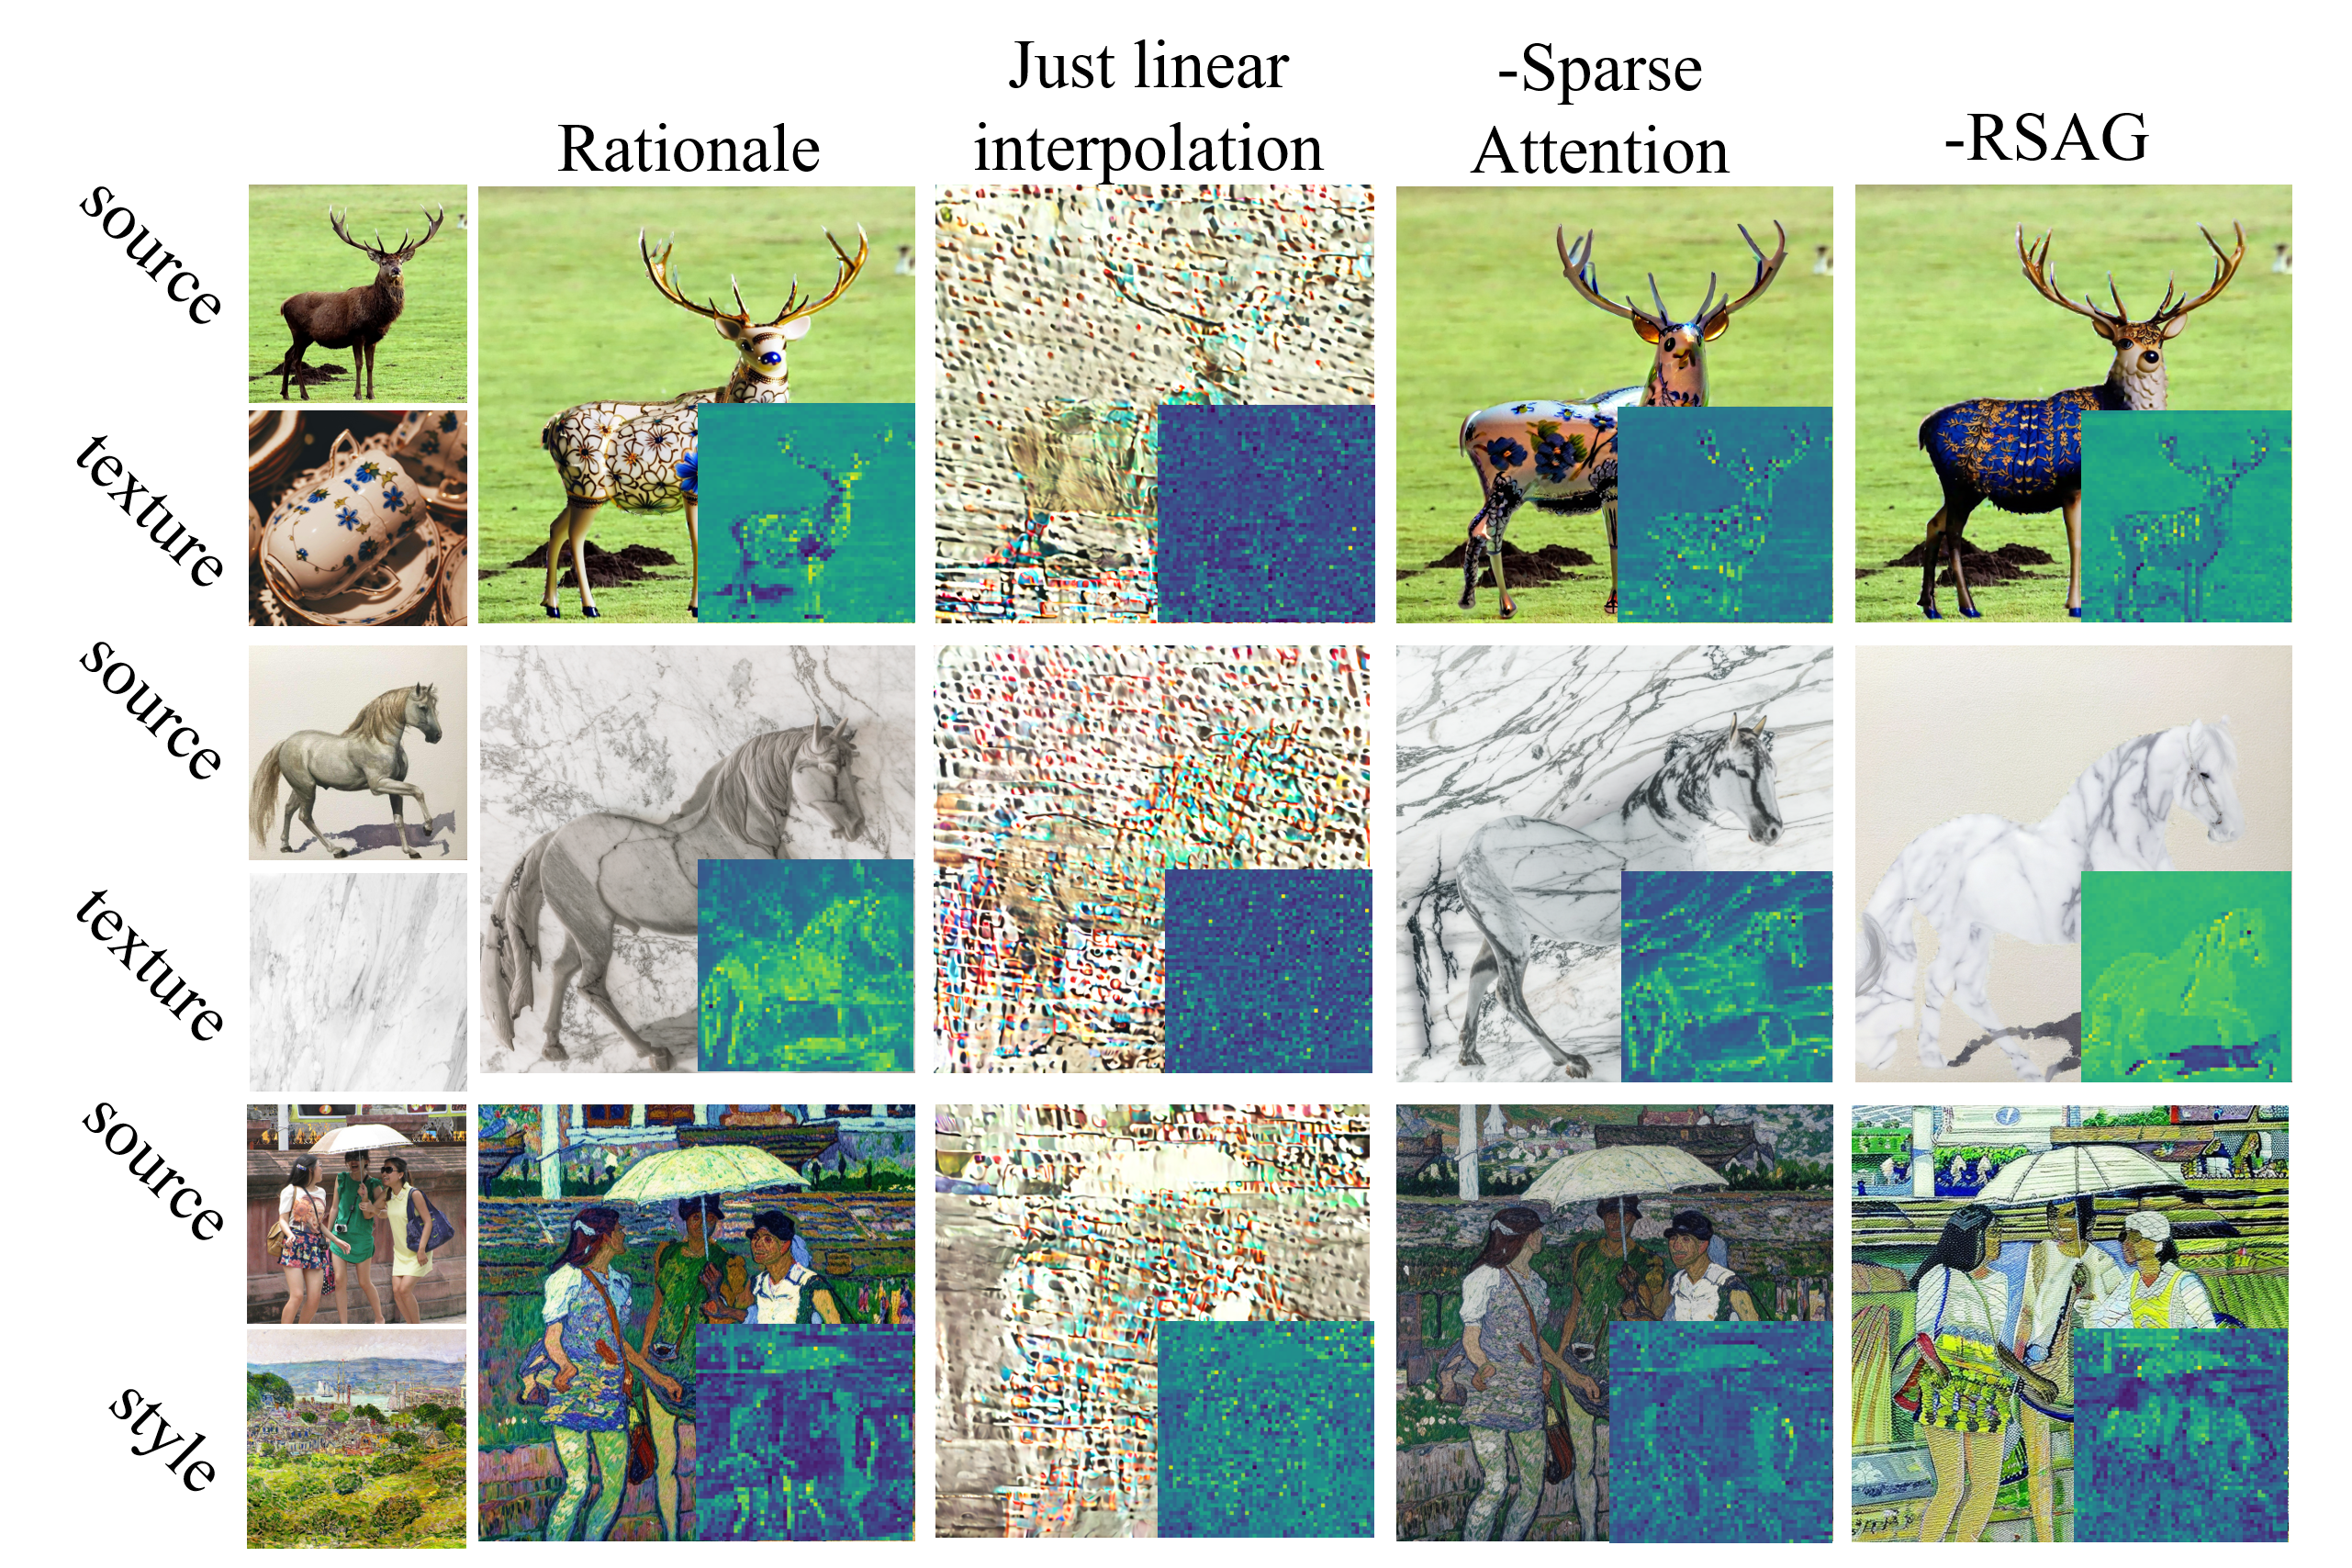
\includegraphics[width=1.0\columnwidth]{images/ablation.png}
    \caption{Qualitative results of the ablation study.}
    \label{fig:ablation}
\end{figure}




\subsection{Parameter Analysis and Controllability}
\label{subsec:parameter}

Finally, we analyze the model's sensitivity to key parameters and demonstrate its high degree of controllability, a crucial feature for artistic and practical applications.


\begin{figure}[htbp]
    \centering
    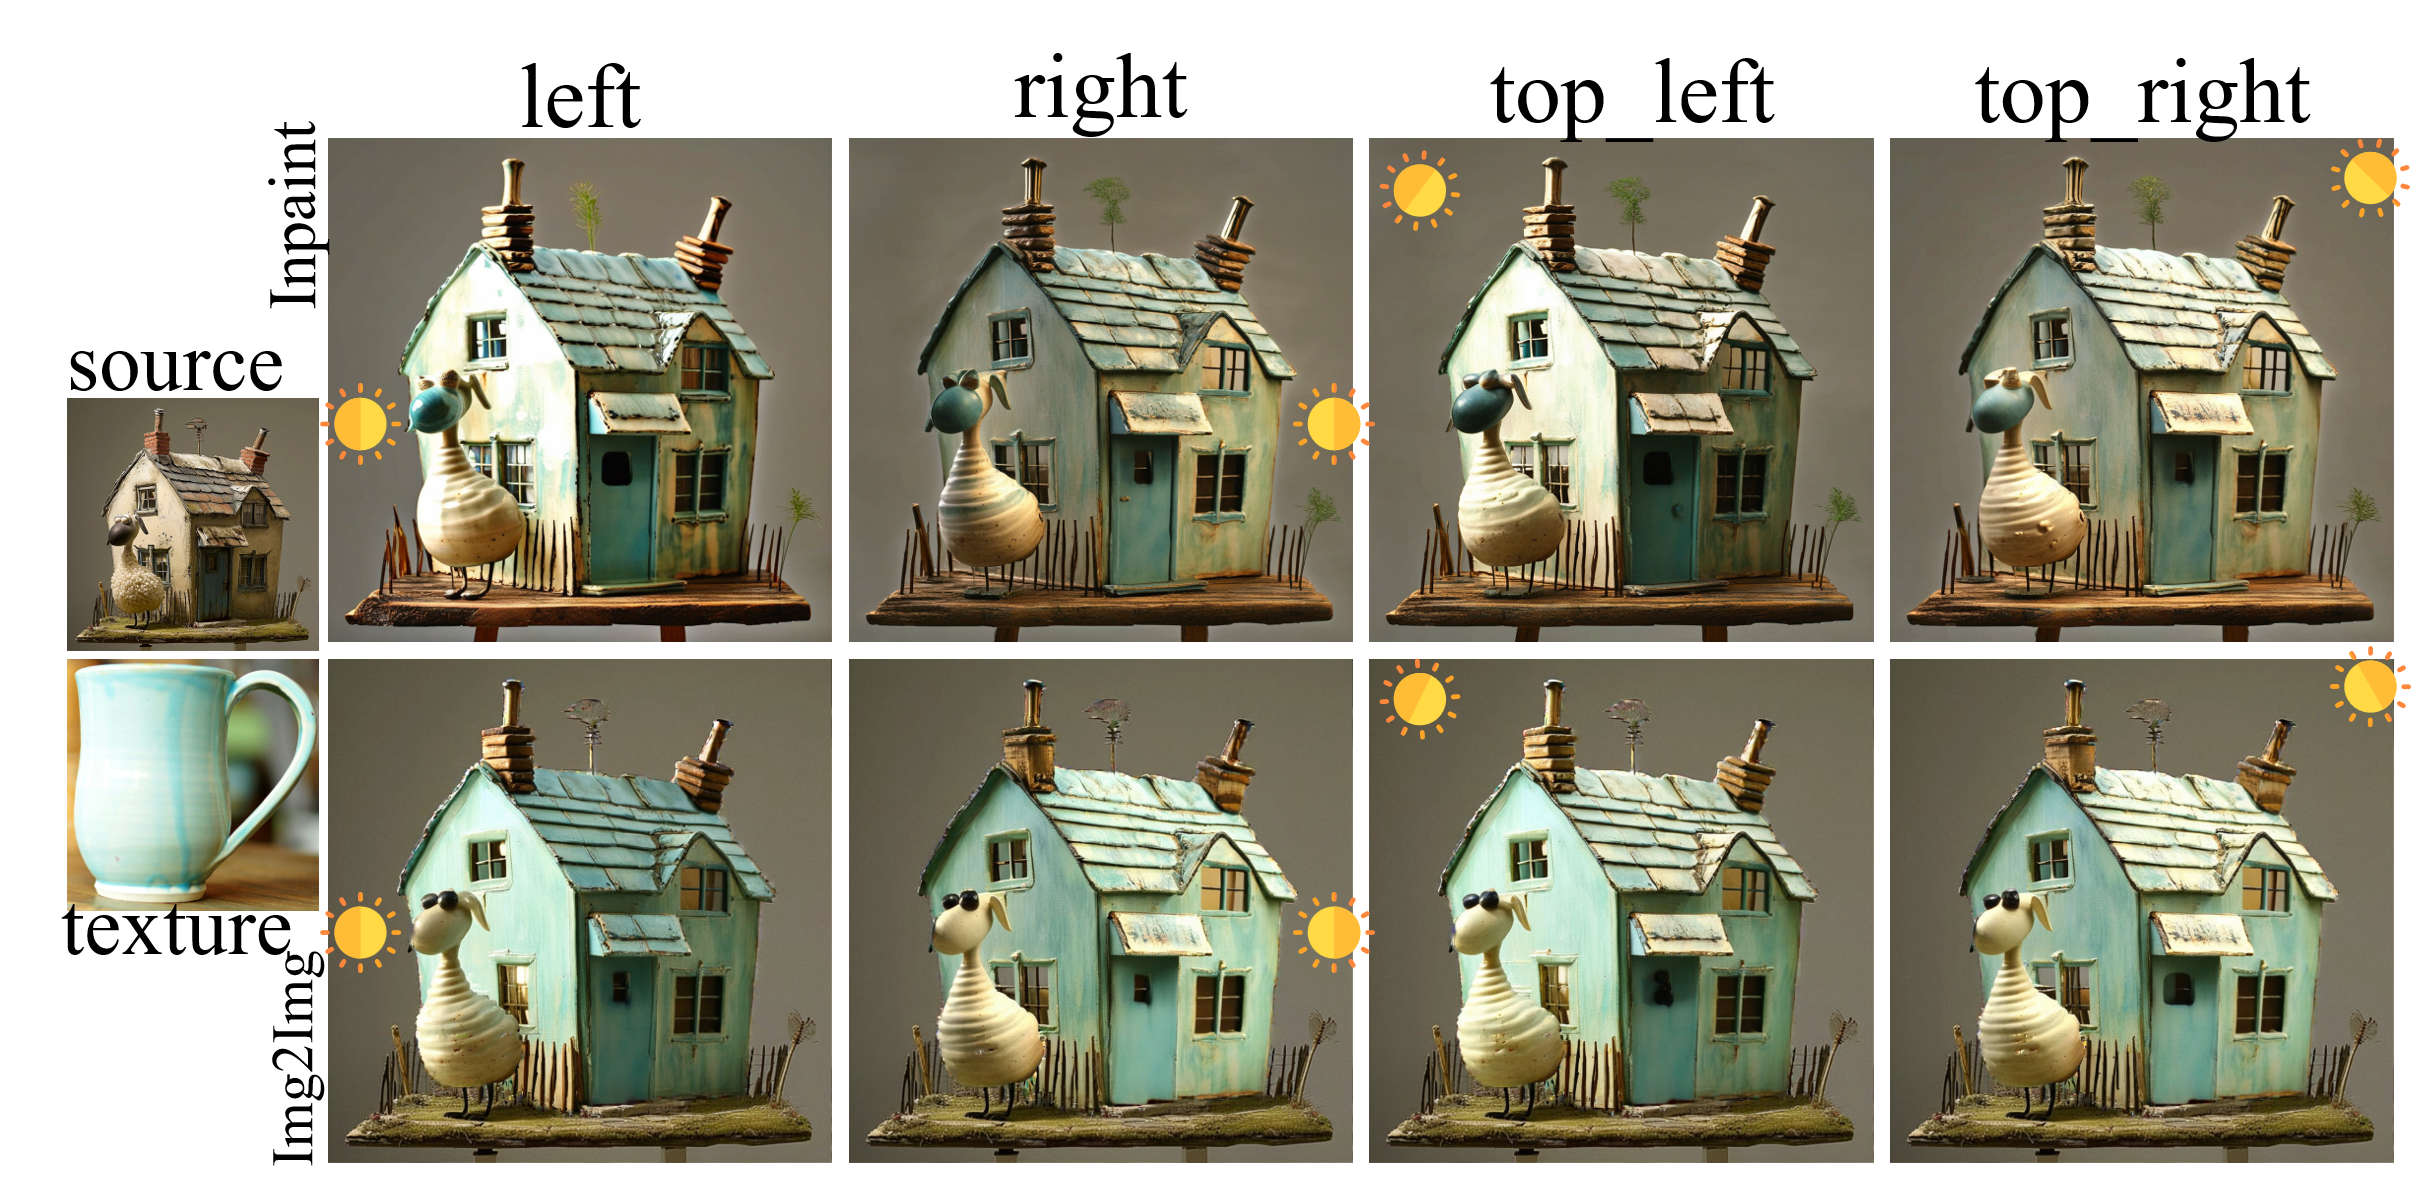
\includegraphics[width=1.0\columnwidth]{images/lighting_direction.png}
    \caption{Demonstration of lighting control by changing the virtual light source direction. Please zoom in for detals.}
    \label{fig:lighting_direction}
\end{figure}


\noindent\textbf{Lighting Control.} Demonstrating a sophisticated, 3D-aware understanding, our model allows for explicit control over the lighting environment. Figure~\ref{fig:lighting_direction} shows how manipulating the virtual light source direction produces realistic and corresponding changes in highlights and shadows.


\noindent\textbf{Structural Intensity Control.} To modulate the prominence of structural features, we introduce a scale parameter, $\gamma$. As illustrated in Figure~\ref{fig:structure}, adjusting $\gamma$ allows for fine-grained control over structural enhancement. The corresponding attention maps further validate this, clearly showing that the model's focus on structural features intensifies as the scale $\gamma$ increases.
